
\begin{parag}{Example}
    Let $f\left(z\right) = z \sin\left(\frac{1}{z}\right)$, the claim is that this function has an essential singularity at $0$.\\
	$ $\\
	Indeed, we can realise this by using the Taylor expansion for this sin function which will gives us a Laurent series:
	\begin{align*} 
		\sin\frac{1}{z} = \sum_{n= 0}^{\infty}\frac{\left(-1\right)^{k}}{\left(2n + 1\right)!}\left(\frac{1}{z}\right)^{n+1}
	\end{align*}
	And hence, by multiplying this sum by $z$:
	\begin{align*} 
		z \sin\frac{1}{z} = \sum_{n= 0}^{\infty}\frac{\left(-1\right)^{n}}{\left(2n + 1\right)!}\frac{1}{z^{2n}}
	\end{align*}
	And this indeed converges when $z\neq 0$.
\end{parag}

\section{Residues}
A residue is a very simple object: it is the first coefficient of the Laurent series
\begin{definition}{Residue}
	The coefficient $c_{-1}$ of the term $\left(z - z_0\right)^{-1}$ in the Laurent series for $f$ at $z_0$ is called the \important{residue} of $f$ at $z_0$. Denoted by:
	\begin{align*} 
		\text{Res}_{z_0}\left(f\right) := c_{-1}
	\end{align*}
\end{definition}
\begin{framedremark}\label{rem:definitionRes}
We have already seen that the coefficients of the Laurent series can be described directly using line integral.
\begin{align*} 
	\text{Res}_{z_0}\left(f\right) = \frac{1}{2\pi i}\int_{\gamma}f\left(z\right)dz
\end{align*}
Where $\gamma$ is a closed, simple, counterclockwise oriented curve that contains $z_0$ in its interior and $f$ is holomorphic on the int $\gamma \setminus \left\{z_0\right\}$
\end{framedremark}

Now let us compute some residue!!!!!!!!!!!!!!!!!!

\begin{parag}{Example}
    If $f$ is holomorphic on an open set containing $z_0$,
	\begin{align*} 
		\text{Res}_{z_0} \left(f\right) = 0
	\end{align*}
	By Cauchy's theorem\\
	$ $\\

The concept of residue becomes interesting when we have singularity inside our function, especially at $0$. For instance if we take:
\begin{align*} 
	\text{Res}_{z_0}\left(\frac{1}{z}\right)
\end{align*}
Then we can see that we already have the Laurent series of $\frac{1}{z}$ at the point $0$.

\begin{align*} 
	\text{Res}_{z_0}\left(\frac{1}{z}\right) = 1
\end{align*}

    Suppose more generally $f$ has a pole of order $m$ at $z_0$, i.e. its Laurent series reads
	\begin{align*} 
		f\left(z\right) = c_{-m}\left(z - z_0\right)^{-m} + \cdots + c_{-1}\left(z - z_0\right)^{-1} + c_0 + \cdots
	\end{align*}
	Where $c_{-m} \neq 0$, consider the holomorphic function
	\begin{align*} 
		g\left(z\right) &=  \left(z - z_0\right)^{m}f\left(z\right)\\
						&=  c_{-m} + c_{-m + 1}\left(z - z_0\right) + \cdots + c_{-1}\left(z -z_0\right)^{m - 1} + \cdots
	\end{align*}
	Then we can extract the residue by the formula 
	\begin{align*} 
		c_{-1} &= \frac{1}{\left(m - 1\right)!} \frac{d^{m-1}}{dz^{m-1}} \eval_{z_0}\left(z\right)\\
		&= \lim_{z  \to z_0}  \frac{1}{\left(m - 1\right)!}\frac{d^{m-1}}{dz^{m-1}}\left(\left(z - z_0\right)^{m}f\left(z\right)\right)
	\end{align*}
	This formula is useful if we already know that $f$ has a pole of order $m$ at $z_0$. In particular if $m = 1$ then this becomes
	\begin{align*} 
		\text{Res}_{z_0}\left(f\right) =  \lim_{z  \to z_0} \left(z - z_0\right)f\left(z\right)
	\end{align*}

\end{parag}


\begin{parag}{Example}
    Let us consider $f\left( z\right) = \frac{1}{\sin z}$ at $z_0 = 0$ which has a pole of order $1$:
	\begin{align*} 
		f\left(z\right) =  \left[z - \frac{z^3}{3!} + \cdots\right]^{-1} = \frac{1}{z}\underbrace{\left[1 - \frac{z^2}{3!} + \cdots\right]^{-1}}_{\text{regular}} 
	\end{align*}
	Hence from the above example, 
	\begin{align*} 
		\text{Res}_0 \left(f\right) &=  \lim_{z \to 0}  zf\left(z\right)\\
									&= \lim_{z  \to 0} \frac{z}{\sin z}\\
									&= \lim_{z \to  0} z \left[z - \frac{z^3}{3!} + \cdots\right]^{-1} \\
									&=  \lim_{z \to 0} \left[1 - \frac{z^2}{3!} + \cdots\right]^{-1} = 1
	\end{align*}
\end{parag}


\subsection{Residue Theorem}
\begin{theoreme}
	Suppose $D \subseteq \mathbb{C}$ is an open and simply connected set and let $\gamma$ be a simple closed curve in $D$ which is counterclockwise oriented. Let $z_1, \ldots, z_m \in \text{ int}\gamma$.\\
	$ $\\
	Assume $f : D \setminus \left\{z_1, \ldots, z_m\right\} \to \mathbb{C}$ is holomorphic\\
	$ $\\
	then 
	\begin{align*} 
		\int_{\gamma}f\left(z\right)dz = 2\pi i \left[\text{Res}_{z_1}\left(f\right) + \cdots + \text{Res}_{z_m}\left(f\right)\right]
	\end{align*}
\end{theoreme}

	\begin{center}
	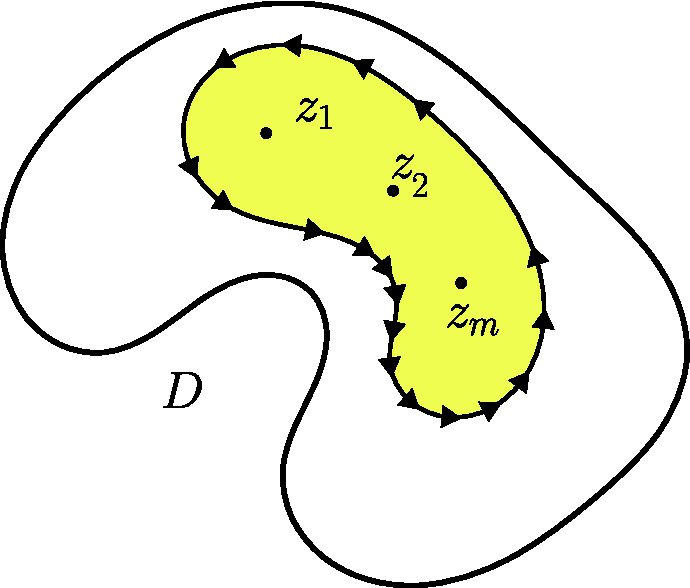
\includegraphics[width=0.4\textwidth]{figure/2026-03-26.pdf}
	\end{center}

	Hence, in order to compute the line integral of $\int_{\gamma}fdz$ it suffices to compute the residues of the singular points in the interior of $\gamma$.

	\begin{parag}{How does one show this?}
	    For simplicity, we will consider for $2$ points only (the same argument foes for $n$ points)\\
		$ $\\
		What we are doing geometrically is creating two curves $\rho_1, \rho_2$ that turns around $z_1$ and $z_2$ and join them together with a very small line, geometrically this gives us something like this:
		\begin{center}
		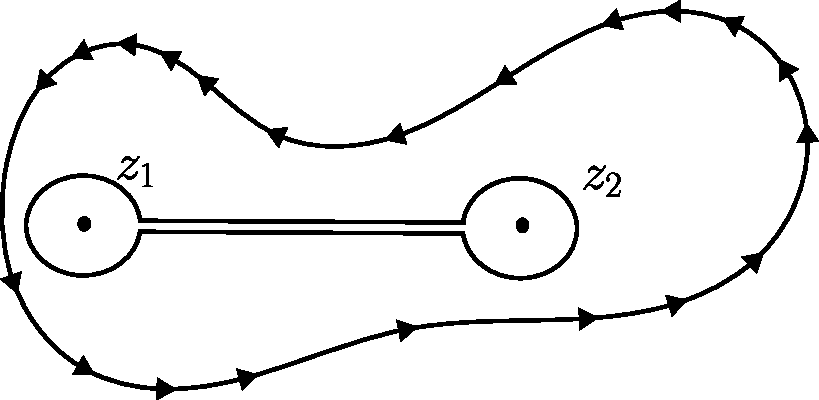
\includegraphics[width=0.4\textwidth]{figure/2026-03-26_1.pdf}
		\end{center}
		By the extension of Cauchy's theorem 
		\begin{align*} \int_{\gamma}fdz =  \int_{\rho}fdz \end{align*}
		Then we are trying to see what happens with the integral of $\rho$ when the radius becomes very thin. First, for the '\textit{bridge}', as it becomes very narrow, it will cancel out. This leaves us with the integral over $\rho_1, \rho_2$. Therefore
		\begin{align*} 
			\int_{\gamma}fdz =  \int_{\rho_1}fdz + \int_{\rho_2}fdz = 2\pi i \text{Res}_{z_1}\left(f\right) + 2\pi i \text{Res}_{z_2}\left(f\right)
		\end{align*}
		\begin{subparag}{Remark}
		    Recall that:
			\begin{align*} 
				\int_{\rho_1}fdz =  2\pi i \text{Res}_{z_1}\left(f\right)
			\end{align*}
			Comes down from the definition of the Residue seen in the Remark~\ref{rem:definitionRes}.
		\end{subparag}
	\end{parag}


	\begin{parag}{Example}
	    Consider $f\left(z\right) =  \frac{1}{z}$. Let $\gamma$ be a simple closed counterclockwise curve in $\mathbb{C}$. Compute $\int_{\gamma}fdz$
		\begin{enumerate}
		    \item If $0 \in$ int $\gamma$ then by the residue theorem 
				\begin{align*} \int_{\gamma}fdz = 2\pi i Res_{0}\left(f\right) = 2\pi i \end{align*}
				\item If $0 \notin$ int $\gamma \cup \gamma$ then 
					\begin{align*} \int_{\gamma} fdz = 0 \end{align*}
					\item if $0 \in \gamma$ then 
						\begin{align*} 
							\int_{\gamma} fdz \text{ is not well-defined}
						\end{align*}
		\end{enumerate}
		
	\end{parag}
	\begin{parag}{Example}
		Let $f  : \mathbb{C} \setminus \left\{0, -1\right\} \to \mathbb{C}$, $f\left(z\right) = \frac{1}{z\left(z + 1\right)} $. We have already seen $f$ has two poles of order 1 at $z_0 = 0$ and $z_1 =  -1$. Hence

		\begin{align*} 
			\text{Res}_{0}\left(f\right) = \lim_{z \to 0} zf\left(z\right)  = \lim_{z \to 0} \frac{1}{z + 1} = 1\\
			\text{Res}_{-1}\left(f\right) =  \lim_{z \to -1} \left(z + 1\right)f\left(z\right) =  \lim_{z \to -1} \frac{1}{z} = -1

		\end{align*}
		Let $\gamma$ be a \si\mple closed counterclockwise oriented curve. The que\astion is always the same: what is $\int_{\gamma}fdz$?
		\begin{enumerate}
		    \item 0, $-1 \notin $ int $\gamma \cup \gamma$ then $\int_{\gamma}fdz = 0$
		    \item $0 \in \text{ int}\gamma$ but $-1 \notin $ int $\gamma \cup \gamma$ then 
				\begin{align*} 
					\int_{\gamma}fdz =  2\pi i \text{Res}_0\left(f\right) = 2\pi i 
				\end{align*}
				\item $0 \notin $int $\gamma \cup \gamma$ but $-1 \in $ int $\gamma$ then 
					\begin{align*} 
						\int_{\gamma}fdz =  2\pi i \text{Res}_{-1}\left(f\right) = -2\pi i
					\end{align*}
					\item If $0, -1 \in $ int $\gamma$ then by the residue theorem 
						\begin{align*} 
							\int_{\gamma}fdz = 2\pi i \left[\text{Res}_0\left(f\right) + \text{Res}_{-1}\left(f\right)\right] = 0
						\end{align*}
					\item $0 \in \gamma$ or $-1 \in \gamma$ then the integral is not well defined
		\end{enumerate}
		What is important is that when we are asked to compute simple line integral, it is important the divide cases based the singularities inside of $\gamma$
	\end{parag}

	\begin{parag}{Example}
	    Let $f : \mathbb{C} \setminus \left\{0, 1\right\} \to \mathbb{C}$, $f\left(z\right) =  \frac{1}{z^2} + \frac{2}{z} + \frac{3}{z - 1}$. This function has a pole of order $2$ at $0$ and a pole of order $1$ at $1$
	\end{parag}
\begin{parag}{Example}
    Let $\exp\left(\frac{1}{z^2}\right) =  1 = \frac{1}{z^2} + 1\frac{1}{2!}\frac{1}{z^2} + \cdots$ hence 
	\begin{align*} 
		\text{Res}_0\left(\exp\left(\frac{1}{z^2}\right)\right) =  0
	\end{align*}
\end{parag}

\subsection{Applications}

The residue theorem can be used to compute integrals over simple closed curve, sometimes even to compute \important{real} integral by replacing them with complex integrals.


\begin{parag}{Example}
	Let us for instance compute 
	\begin{align*} 
		\int_{-\infty}^{\infty} \frac{1}{1 + x^2} dx
	\end{align*}
	If you have forgotten that this is the primitive of $\arctan$ then you can still try to rephrase this into a complex integral. Let us set $f\left(z\right) =  \frac{1}{1 + z^2}$.\\
	$ $\\
	Given $R > 0$, consider the segment $L_R: \left[-R, R\right] \to \mathbb{C}$ given by $L_R\left(t\right) = t$ and the half circle $c_R : \left[0, \pi\right] \to \mathbb{C}$ given by $C_R\left(t\right) =  Re^{it}$\\
	$ $\\
	Consider the closed curve $\gamma = LR \cup C_R$. Then the function $f\left(z\right) = \frac{1}{1 + z^2}$ has poles of order $1$ at $i$. From the residue theorem then 
	\begin{align*} 
		\int_{\gamma} fdz =  2\pi i \text{Res}_i \left(f\right)
	\end{align*}
	But we can compute the residue explicitly which is given by 
	\begin{align*} \text{Res}_i\left(f\right) =  \lim_{z  \to i} \left(z - i\right)f\left(z\right) =  \lim_{z \to i} \frac{1}{z + i} = \frac{1}{2i} \end{align*}


	So:
	\begin{align*} 
		\int_{\gamma} ddz =  \pi &=  \int_{L_R}fdz + \int_{C_R}fdz\\
		&= \int_{-R}^{R} \frac{1}{1 + t^2}dt \underbrace{\to}_{R \to \infty} \int_{-\infty}^{\infty}\frac{1}{1 + t^2}dt
	\end{align*}
	On the other hand, 
	\begin{align*} 
		\int_{C_R}fdz =  \int_0^{\pi} \frac{1}{1 + R^2e^{2it}}Rie^{it}dt \approx \frac{\pi}{R} \underbrace{\to}_{R \to \infty}
	\end{align*}
	This method works for any integrand that decays faster than $\frac{1}{R}$ as $R \to \infty$
\end{parag}

\begin{parag}{Example}
    Let $R\left(x\right) = \frac{P\left(x\right)}{Q\left(x\right)}$ where $P, Q$ are real polynomials and deg $Q \geq$ deg $P + 2$. Assume $R$ is defined on $ \mathbb{R}$ which means that $Q\left(x\right) \neq 0 \mathspace \forall x \in \mathbb{R}$
	\begin{subparag}{Observations}
	    \begin{enumerate}
	        \item The latter condition on $Q$ forces deg $Q$ to be even
	        \item $Q$ has real coefficients if $Q\left(z\right) = 0$ for $z \in \mathbb{C}$ then by taking the complex conjugate of this equations, we find $Q\left(\overline{z}\right) = 0$ So roots of $Q$ in $\mathbb{C}$ come in pairs of complex conjugates (none of which are real)
	    \end{enumerate}
	    
	\end{subparag}
\end{parag}



	
	
	
	
	



